\documentclass[11pt]{article}
\usepackage{amsmath,amsfonts,amssymb,amsthm,epsfig}
\usepackage[left=2cm, right=2cm, top=2cm, bottom=2cm]{geometry}

\usepackage{xcolor}
\usepackage{fp}
\usepackage{tikz}
\usetikzlibrary{cd}
\usetikzlibrary{knots}
\usetikzlibrary{calc}

\usetikzlibrary{matrix}
\usetikzlibrary{arrows,backgrounds,patterns,scopes,external,hobby,
    decorations.pathreplacing,
    decorations.pathmorphing
}

\tikzset{use Hobby shortcut}


\tikzset{string/.style={ultra thick}}
\tikzset{smallstring/.style={thick,scale=0.75,every node/.style={transform shape}}}
\tikzset{
    triple/.style args={[#1] in [#2] in [#3]}{
        #1,preaction={preaction={draw,#3},draw,#2}
    }
}
\tikzset{
    quadruple/.style args={[#1] in [#2] in [#3] in [#4]}{
        #1,preaction={preaction={preaction={draw,#4},draw,#3}, draw,#2}
    }
} 
\tikzset{
	super thick/.style={line width=3pt},
	more thick/.style={line width=1pt},
}

\usepackage{graphicx}
\usepackage[T1]{fontenc}
\usepackage[final]{microtype}
\usepackage{libertine}
\usepackage[libertine]{newtxmath}
\usepackage[all]{xy}


% Theorems
\theoremstyle{plain}
\newtheorem{theorem}{Theorem}
\newtheorem{proposition}{Proposition}
%\numberwithin{proposition}{section}
\newtheorem{lemma}[proposition]{Lemma}
\newtheorem{corollary}[proposition]{Corollary}
\newtheorem{claim}[proposition]{Claim}
\newtheorem{conjecture}[proposition]{Conjecture}
\newtheorem{observation}[proposition]{Observation}
\newtheorem{warning}[proposition]{Warning}

\theoremstyle{definition}
\newtheorem{definition}[proposition]{Definition}
\newtheorem{exercise}[proposition]{Exercise}
\newtheorem{question}[proposition]{Question}
\newtheorem{problem}[proposition]{Problem}

\theoremstyle{remark}
\newtheorem{example}[proposition]{Example}
%\newtheorem{hint}[proposition]{Hint}
\newtheorem{remark}[proposition]{Remark}
%\newtheorem{apology}[proposition]{Apology}
%\newtheorem{warning}[proposition]{Warning}

\newcommand{\fdVec}{\mathsf{fdVec}}
\renewcommand{\Vec}{\mathsf{Vec}}
\newcommand{\Rep}{\mathsf{Rep}}
\newcommand{\Mat}{\mathsf{Mat}}

% tricky way to iterate macros over a list
\def\semicolon{;}
\def\applytolist#1{
    \expandafter\def\csname multi#1\endcsname##1{
        \def\multiack{##1}\ifx\multiack\semicolon
            \def\next{\relax}
        \else
            \csname #1\endcsname{##1}
            \def\next{\csname multi#1\endcsname}
        \fi
        \next}
    \csname multi#1\endcsname}

% \def\cA{{\cal A}} for A..Z
\def\calc#1{\expandafter\def\csname c#1\endcsname{{\mathcal #1}}}
\applytolist{calc}QWERTYUIOPLKJHGFDSAZXCVBNM;
% \def\bbA{{\mathbb A}} for A..Z
\def\bbc#1{\expandafter\def\csname bb#1\endcsname{{\mathbb #1}}}
\applytolist{bbc}QWERTYUIOPLKJHGFDSAZXCVBNM;
% \def\bfA{{\mathbf A}} for A..Z
\def\bfc#1{\expandafter\def\csname bf#1\endcsname{{\mathbf #1}}}
\applytolist{bfc}QWERTYUIOPLKJHGFDSAZXCVBNM;
 
 
\begin{document}
\title{Homework on monoidal categories}
\maketitle

\begin{exercise}
Show that $\fdVec$ and $\Mat$ are equivalent as categories.
\end{exercise}
\begin{proof}[Hint:]
Pick a basis for every finite dimensional vector space.
\end{proof}

\begin{exercise}
Show that every category is equivalent to a skeletal category.
\end{exercise}

\begin{exercise}
Show that $TL(d=1)$ is monoidally equivalent to $\Rep(\bbZ / 2 \bbZ)$.
\end{exercise}

\begin{exercise}
If $\cC$ is a monoidal category, $\cD$ is a category, and we have an equivalence $F:\cC \leftrightarrow \cD:G$, show you can make $D$ into a tensor monoidal in such a way that $F$ and $G$ are a monoidal equivalence.
\end{exercise}
(This is an instance of the idea of `transport of structure`.)

\begin{exercise}
Conclude that every monoidal category is equivalent to a skeletal monoidal category. 
\end{exercise}

\begin{exercise}
Recall that a monoidal functor is a pair: a functor and a natural isomorphism $F(X \otimes Y) \to F(X) \otimes F(Y)$.  Classify all monoidal functors from $\Vec(G)$ to $\Vec(G)$ where the underlying functor is the identity functor. 
\end{exercise}
\begin{proof}[Hint:]
Your answer should involve group cohomology of $G$.
\end{proof}

\begin{exercise}
Find the fusion rules for $TL(q+q^{-1})$ at $q$ a root of unity.

Conclude that the last surviving Jones-Wenzl idempotent is invertible.  This gives a 2-object subcategory where all the objects are invertible --- how does it fit into our classification?
\end{exercise}
\begin{proof}[Hint:]
Suppose we are a root of unity such that $f^{(n+1)}$ is the first negligible Jones-Wenzl idempotent. Prove that $f^{(k)} \otimes f^{(1)} \cong f^{(k-1)} \oplus f^{(k+1)}$ unless $k=0$ or $k=n$. What happens in those cases? From these observations, give a formula for how $f^{(a)} \otimes f^{(b)}$ breaks up as a direct sum of Jones-Wenzl idempotents.
\end{proof}

\begin{exercise}
Show that the golden category, as defined in lecture, is semisimple with two simple objects $1$ and $X$ and in particular that  $X\otimes X \oplus 1 \oplus X$.
\end{exercise}
Recall that the golden category has as objects finite subsets of an interval, and the morphisms are planar trivalent graphs modulo the local relations
\newcommand{\drawI}{ 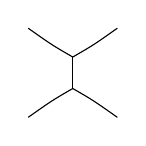
\begin{tikzpicture}[baseline=0cm]
 	\draw (0,.2) .. controls +(30:.3cm) .. (45:.8cm);
 	\draw (0,.2) .. controls +(150:.3cm) .. (135:.8cm);
	\draw (0,.2) -- (0,-.2);
 	\draw (0,-.2) .. controls +(-30:.3cm) .. (-45:.8cm);
 	\draw (0,-.2) .. controls +(-150:.3cm) .. (-135:.8cm);
\end{tikzpicture}
}

\newcommand{\drawH}{ 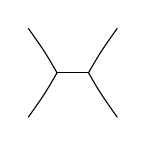
\begin{tikzpicture}[baseline=0cm,rotate=90]
 	\draw (0,.2) .. controls +(30:.3cm) .. (45:.8cm);
 	\draw (0,.2) .. controls +(150:.3cm) .. (135:.8cm);
	\draw (0,.2) -- (0,-.2);
 	\draw (0,-.2) .. controls +(-30:.3cm) .. (-45:.8cm);
 	\draw (0,-.2) .. controls +(-150:.3cm) .. (-135:.8cm);
\end{tikzpicture}}

\newcommand{\cupcap}{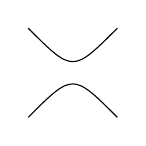
\begin{tikzpicture}[baseline=0cm]
	\draw (45:.8cm) .. controls (0,0) .. (135:.8cm);
	\draw (-45:.8cm) .. controls (0,0) .. (-135:.8cm);
\end{tikzpicture}}

\newcommand{\twostrandid}{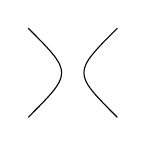
\begin{tikzpicture}[baseline=0cm,rotate=90]
	\draw (45:.8cm) .. controls (0,0) .. (135:.8cm);
	\draw (-45:.8cm) .. controls (0,0) .. (-135:.8cm);
\end{tikzpicture}}

\newcommand{\unknot}{

\begin{tikzpicture}[baseline=-0.5ex,scale=0.8]
  \draw (0,0) circle (.6cm);
\end{tikzpicture}
}

\newcommand{\loopvertex}{

\begin{tikzpicture}[baseline=-0.5ex,scale=0.8]
  \draw (0,-0.5)--(0,-0.8);
  \draw ([out angle=150]0,-0.5)..(-0.02,0.6)..(0.02,0.6)..([in angle=30]0,-0.5);
\end{tikzpicture}
}

\begin{align*}
\unknot\; &= d \\ 
    \loopvertex\;&=0\\
\drawI \; & = \; \twostrandid \; -  \frac{1}{d}\; \cupcap
\end{align*}

\begin{exercise}
(Checking every detail here is tedious; use your judgement!)

Show that every monoidal category $\cC$ is monoidally equivalent to the strict monoidal category $\mathsf{List} \cC$.

Here $\mathsf{List} \cC$ has as objects words in the objects of $\cC$, and $$\mathsf{List} \cC([x_1, x_2, \ldots x_n] \to [y_1, y_2, \ldots y_m]) = \cC(x_1 \otimes (x_2 \otimes \cdots \otimes (x_n \otimes 1)) \to y_1 \otimes (y_2 \otimes \cdots \otimes (y_m \otimes 1))).$$ Part of the exercise is to define the tensor product of morphisms in $\mathsf{List} \cC$. The functors between $\cC$ and $\mathsf{List} \cC$ should send $x$ to $[x]$ and $[x_1, x_2, \ldots x_n]$ to $x_1 \otimes (x_2 \otimes \cdots \otimes (x_n \otimes 1))$. You'll need to specify what the functors do on morphisms, and make them into monoidal functors by specifying tensorators. Finally you'll need to show that these functors form an equivalence; you can do this directly, or show one of the functors is fully faithful and essentially surjective.
\end{exercise}

\end{document}